\documentclass[a4paper,11pt]{article}
\input{/home/tof/Documents/Cozy/latex-include/preambule_doc.tex}
\input{/home/tof/Documents/Cozy/latex-include/preambule_commun.tex}
\newcommand{\showprof}{show them}  % comment this line if you don't want to see todo environment
\setlength{\fboxrule}{0.8pt}
\fancyhead[L]{\fbox{\Large{\textbf{ArchMat 02}}}}
\fancyhead[C]{\textbf{Programmation assembleur}}
\newdate{madate}{10}{09}{2020}
%\fancyhead[R]{\displaydate{madate}} %\today
\fancyhead[R]{Première - NSI}
\fancyfoot[L]{\vspace{1mm}Christophe Viroulaud}
\AtEndDocument{\label{lastpage}}
\fancyfoot[C]{\textbf{Page \thepage/\pageref{lastpage}}}
\fancyfoot[R]{\includegraphics[width=2cm,align=t]{/home/tof/Documents/Cozy/latex-include/cc.png}}

\begin{document}
L'\emph{unité de contrôle} d'un processeur lit des instructions contenues dans la mémoire et ordonne à l'\emph{unité arithmétique et logique} de les exécuter.
\begin{center}
    \framebox{Comment l'Homme communique avec la machine?}
\end{center}
\section{Langage machine}
\begin{aretenir}[]
    Un processeur est un composant électronique: il n'interprète que des signaux électriques.
\end{aretenir}
Un processeur ne peut exécuter que des instructions basiques:
    \begin{itemize}
        \item \textbf{opérations arithmétiques:} \emph{\guill{additionne la valeur contenue dans le registre R1 et le nombre 789 et range le résultat dans le registre R0}}
        \item \textbf{transfert de données entre les registres et la mémoire vive:} \emph{\guill{prendre la valeur située à l’adresse mémoire 487 et la placer dans la registre R2}}
        \item \textbf{rupture de séquence:} \emph{\guill{saute de l'instruction 2 à l'instruction 5}}
    \end{itemize}
\section{Langage assembleur}
\subsection{Un langage intermédiaire}
\begin{aretenir}[]
    Pour faciliter la vie des informaticiens, on remplace les code binaires par des \textbf{symboles mnémoniques}.

    \centering ADD, MOV, SUB\dots
\end{aretenir}
\subsection{Découverte d'un simulateur}
\begin{center}
    \centering
    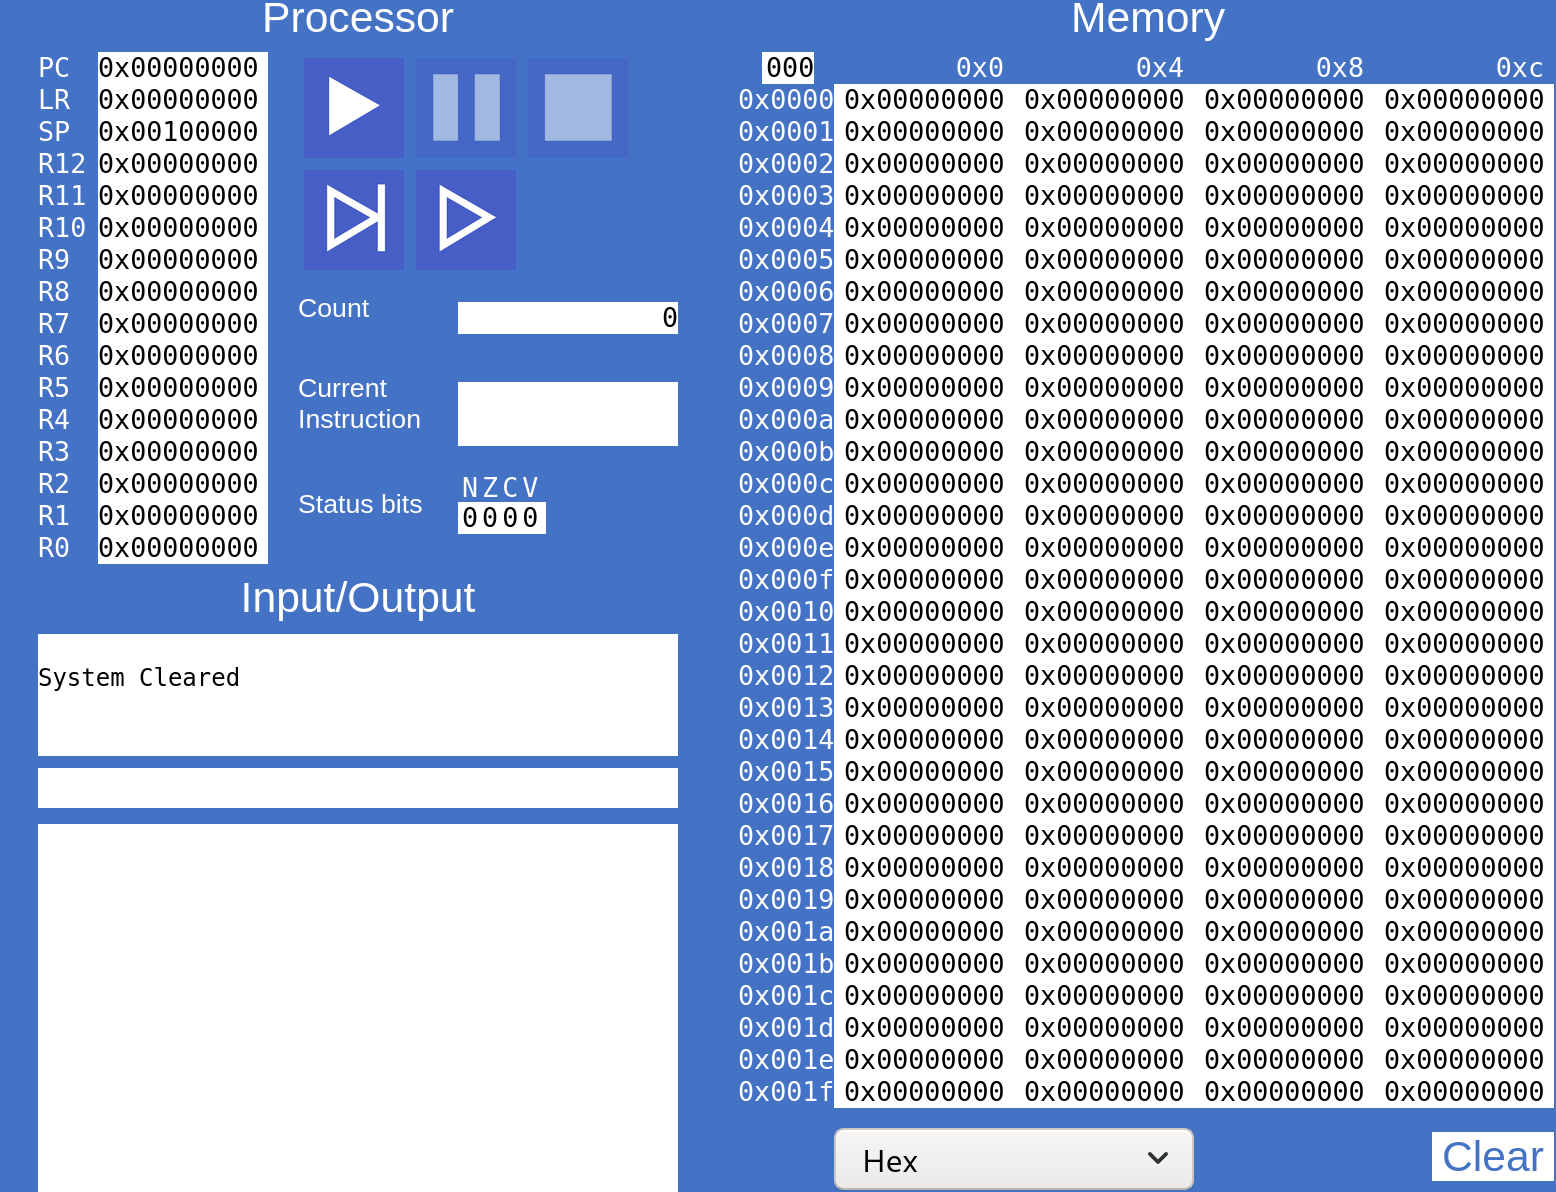
\includegraphics[width=10cm]{ressources/simulateur.png}
    \captionof{figure}{Simulateur 32-bit ARM}
    \label{IMG}
\end{center}
\subsection{Opérations arithmétiques}
\begin{center}
    \begin{lstlisting}[language=C , basicstyle=\small, xleftmargin=2em, xrightmargin=2em]
ADD R0,R1,R2
\end{lstlisting}
    \captionof{code}{Ajoute la valeur du registre R2 à celle de R1 puis place le résultat dans R0.}
    \label{CODE}
\end{center}
\begin{center}
    \begin{lstlisting}[language=C , basicstyle=\small, xleftmargin=2em, xrightmargin=2em]
ADD R1,R1,#10
\end{lstlisting}
    \captionof{code}{Ajoute l'entier 10 à celle du registre R1 puis place le résultat dans R1.}
    \label{CODE}
\end{center}
\subsection{Transfert de données}
\begin{center}
    \begin{lstlisting}[language=C , basicstyle=\small, xleftmargin=2em, xrightmargin=2em]
    MOV R0, #10
\end{lstlisting}
    \captionof{code}{Place la valeur 10 dans R0.}
    \label{CODE}
    \end{center}
    \begin{center}
        \begin{lstlisting}[language=C , basicstyle=\small, xleftmargin=2em, xrightmargin=2em]
LDR R0,16
\end{lstlisting}
        \captionof{code}{\textbf{L}oa\textbf{DR}egister: charge dans R0 la valeur située à \textbf{l'adresse} 16 de la mémoire.}
        \label{CODE}
    \end{center}
    \begin{center}
        \begin{lstlisting}[language=C , basicstyle=\small, xleftmargin=2em, xrightmargin=2em]
STR R0,20
\end{lstlisting}
        \captionof{code}{\textbf{ST}ore\textbf{R}egister: stocke la valeur de R0 dans l'espace mémoire situé à \textbf{l'adresse} 20.}
        \label{CODE}
    \end{center}
\subsection{Rupture de séquence}
    \begin{center}
        \begin{lstlisting}[language=C , basicstyle=\small, xleftmargin=2em, xrightmargin=2em]
    MOV R0, #10
    MOV R1, #10
    // Compare les valeurs de R0 et R1
    CMP R0, R1
    // Si les valeurs sont égales, saute au label
    BEQ labelegal 
    MOV R2, R0
    HALT 
    labelegal: 
    STR R0, mavaleur
    HALT
    mavaleur: 5
\end{lstlisting}
        \captionof{code}{Les \emph{//} permettent de commenter le code.}
        \label{CODE}
        \end{center}
\end{document}